\documentclass[aspectratio=169, 10pt]{beamer}

\usepackage{bm} % bold math
\usepackage{fontspec}
\usepackage{minted}
\usepackage{pgf-pie}
\usepackage{tikz}
\usepackage{graphicx}
\newcommand\sbullet[1][.5]{\mathbin{\vcenter{\hbox{\scalebox{#1}{$\bullet$}}}}}

% Custom commands and environments
\makeatletter
\newcommand\version[1]{\renewcommand\@version{#1}}
\newcommand\@version{}
\def\insertversion{\@version}

\newcommand\course[1]{\renewcommand\@course{#1}}
\newcommand\@course{}
\def\insertcourse{\@course}

\newcommand\coursetitle[1]{\renewcommand\@coursetitle{#1}}
\newcommand\@coursetitle{}
\def\insertcoursetitle{\@coursetitle}

\newcommand\lecturenumber[1]{\renewcommand\@lecturenumber{#1}}
\newcommand\@lecturenumber{}
\def\insertlecturenumber{\@lecturenumber}
\makeatother

\newcommand{\slidetitle}[1]{{\xbseries \large \structure{#1}} \bigskip}
\newcommand{\term}[1]{{\color{blue} #1}}
\newcommand{\leftspace}{\hspace{1em}}
\newcommand{\inlinearrow}{
  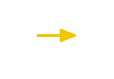
\begin{tikzpicture}[baseline]
    \node [anchor=base] (x) {};
    \draw [rawarrow] (x.mid west) -- ($(x.mid west) + (2em,0)$);
  \end{tikzpicture}
}

\newenvironment{slide}
{\begin{frame}[fragile,environment=slide]\vskip0pt plus 1filll}
{\vskip0pt plus 1filll\end{frame}}

% LaTeX

\setlength{\leftmargini}{1em}

% Common Information

\author{Talia Xu}
\course{COMPSCI 340}
\coursetitle{Operating Systems}
\date{2024 Semester 2}

% fontspec

\defaultfontfeatures{Ligatures=TeX}
% \setmainfont{Domine}
\setsansfont{Inter}[
  FontFace={ul}{n}{Font=*-Thin},
  FontFace={el}{n}{Font=*-ExtraLight},
  FontFace={l}{n}{Font=*-Light},
  FontFace={sb}{n}{Font=*-SemiBold},
  FontFace={eb}{n}{Font=*-ExtraBold},
  FontFace={xb}{n}{Font=*-Black},
]
\setmonofont[Contextuals=AlternateOff, Ligatures=TeXOff]{Iosevka}[
  FontFace={xb}{n}{Font=*-Heavy},
]

%% Font Weights

\DeclareRobustCommand{\ulseries}{\fontseries{ul}\selectfont}
\DeclareTextFontCommand{\textul}{\ulseries}
\DeclareRobustCommand{\elseries}{\fontseries{el}\selectfont}
\DeclareTextFontCommand{\textel}{\elseries}
\DeclareRobustCommand{\lseries}{\fontseries{l}\selectfont}
\DeclareTextFontCommand{\textl}{\lseries}
\DeclareRobustCommand{\sbseries}{\fontseries{sb}\selectfont}
\DeclareTextFontCommand{\textsb}{\sbseries}
\DeclareRobustCommand{\ebseries}{\fontseries{eb}\selectfont}
\DeclareTextFontCommand{\texteb}{\ebseries}
\DeclareRobustCommand{\xbseries}{\fontseries{xb}\selectfont}
\DeclareTextFontCommand{\textxb}{\xbseries}

% tikz

\usetikzlibrary{
  arrows,
  arrows.meta,
  automata,
  backgrounds,
  calc,
  decorations.pathreplacing,
  matrix,
  positioning,
  overlay-beamer-styles,
  shapes,
  shapes.multipart,
  tikzmark,
}

\tikzstyle{rawarrow} = [
  -{Latex[round]},
  line width=1pt,
  yellow,
  shorten >=3pt,
  shorten <=3pt,
  font=\small,
  text=black,
]

\tikzstyle{arrow} = [
  -{Latex[round]},
  line width=1pt,
  yellow,
  shorten >=3pt,
  shorten <=3pt,
  transform canvas={yshift=3pt},
  font=\small,
  text=black,
]

\newcommand{\tikzmarkcoord}[1]{([yshift=3pt]pic cs:#1)}

% minted

\setminted{style=eyolfson, fontsize=\small, escapeinside=||}
\setmintedinline{fontsize=\normalsize}

% hyperref

\hypersetup{colorlinks, urlcolor=blue}

% beamer
\setbeamersize{text margin left=16mm, text margin right=16mm}
\setbeamertemplate{itemize items}[circle]
\setbeamercolor{item}{fg=black}
\setbeamercolor{structure}{fg=darkblue}
\setbeamerfont{frametitle}{series=\bfseries, parent=structure}
\setbeamertemplate{navigation symbols}{}
\setbeamertemplate{headline}{}
\setbeamertemplate{footline}{
  \begin{tikzpicture}[
    remember picture,
    overlay,
    shift={(current page.south west)},
  ]
    \path [fill=gray] (144mm, 0) -- (160mm, 16mm) -- (160mm, 0);
    \node [inner sep=3.5mm, outer sep=0, text=black, anchor=base east,
           align=right, yshift=3.5mm]
          at (current page.south east) {\ttfamily \small \insertframenumber{}};
  \end{tikzpicture}
}
\setbeamertemplate{title page}{
  \begin{tikzpicture}[
    remember picture,
    overlay,
    shift={(current page.south west)},
    background rectangle/.style={fill=darkblue},
    show background rectangle,
  ]
    \node [anchor=center, align=center, text=white, text width=40mm, scale=3.2]
          at (\paperwidth / 2, \paperheight * 2 / 3)
          {\xbseries \inserttitle{}};
    \node [anchor=base west, align=left, inner sep=0, text=white, yshift=2.5mm]
          at (16mm, \paperheight / 3)
          {\insertdate{} \insertcourse{}: \insertcoursetitle{}};
    \node [anchor=base west, align=left, inner sep=0, text=white, yshift=-2.5mm]
          at (16mm, \paperheight / 3)
          {\insertauthor};
    \node [anchor=base east, align=right, inner sep=0, text=white, yshift=2.5mm]
          at (144mm, \paperheight / 3)
          {Lecture \insertlecturenumber{}};
    \node [anchor=base east, align=right, inner sep=0, text=white,
           yshift=-2.5mm]
          at (144mm, \paperheight / 3)
          {\ttfamily \insertversion{}};
    \node [align=center, anchor=south, inner sep=0, text=white, yshift=3.5mm]
          (license) at (\paperwidth / 2, 0)
          {\fontsize{7pt}{7pt}\selectfont This  work is licensed under a
           \href{http://creativecommons.org/licenses/by-sa/4.0/}
                {\color{lightblue} Creative Commons Attribution-ShareAlike 4.0
                 International License}};
  \end{tikzpicture}
}

% xcolor

%% Primary Colour

\definecolor{pantone655}{RGB}{0, 42, 92} % #002a5c
\colorlet{darkblue}{pantone655}

%% Secondary Colours

\definecolor{pantone633}{RGB}{0, 139, 176} % #008bb0
\colorlet{blue}{pantone633}

\definecolor{pantonewarmred}{RGB}{220, 70, 51} % #dc4633
\colorlet{red}{pantonewarmred}

\definecolor{pantone3285}{RGB}{0, 161, 137} % #00a189
\colorlet{cyan}{pantone3285}

\definecolor{pantone7722}{RGB}{13, 83, 77} % #0d534d
\colorlet{darkcyan}{pantone7722}

\definecolor{pantone376}{RGB}{141, 191, 46} % #8dbf2e
\colorlet{green}{pantone376}

\definecolor{pantone2613}{RGB}{109, 36, 122} % #6d247a
\colorlet{violet}{pantone2613}

\definecolor{pantone2985}{RGB}{111, 199, 234} % #6fc7ea
\colorlet{lightblue}{pantone2985}

\definecolor{pantone227}{RGB}{171, 19, 104} % #ab1368
\colorlet{magenta}{pantone227}

\definecolor{pantone7406}{RGB}{241, 197, 0} % #f1c500
\colorlet{yellow}{pantone7406}

%% Neutrals

\definecolor{pantonecoolgray2}{RGB}{208, 209, 201} % #d0d1c9
\colorlet{gray}{pantonecoolgray2}


\lecturenumber{1}
\title{File\\Systems}
\version{1.0.0}

\begin{document}

\begin{frame}[plain, noframenumbering]
    \titlepage
\end{frame}

\begin{slide}
    \slidetitle{To read a file}

    \textbf{The high level idea}
    \begin{itemize}
        \item Perform a path lookup
        \item Traverse the path until we get the file’s inode
        \item The root inode is typically 2 in a Unix file system
        \item Once we have the inode of the file, we can start to read its data
    \end{itemize}
    \bigskip

    Example: We want to read an 8 KB file /foo/bar
\end{slide}

\begin{slide}

    \slidetitle{To read a file}

    Example: We want to read an 8 KB file /foo/bar
    \bigskip

    First we need to open the file.
    \bigskip

    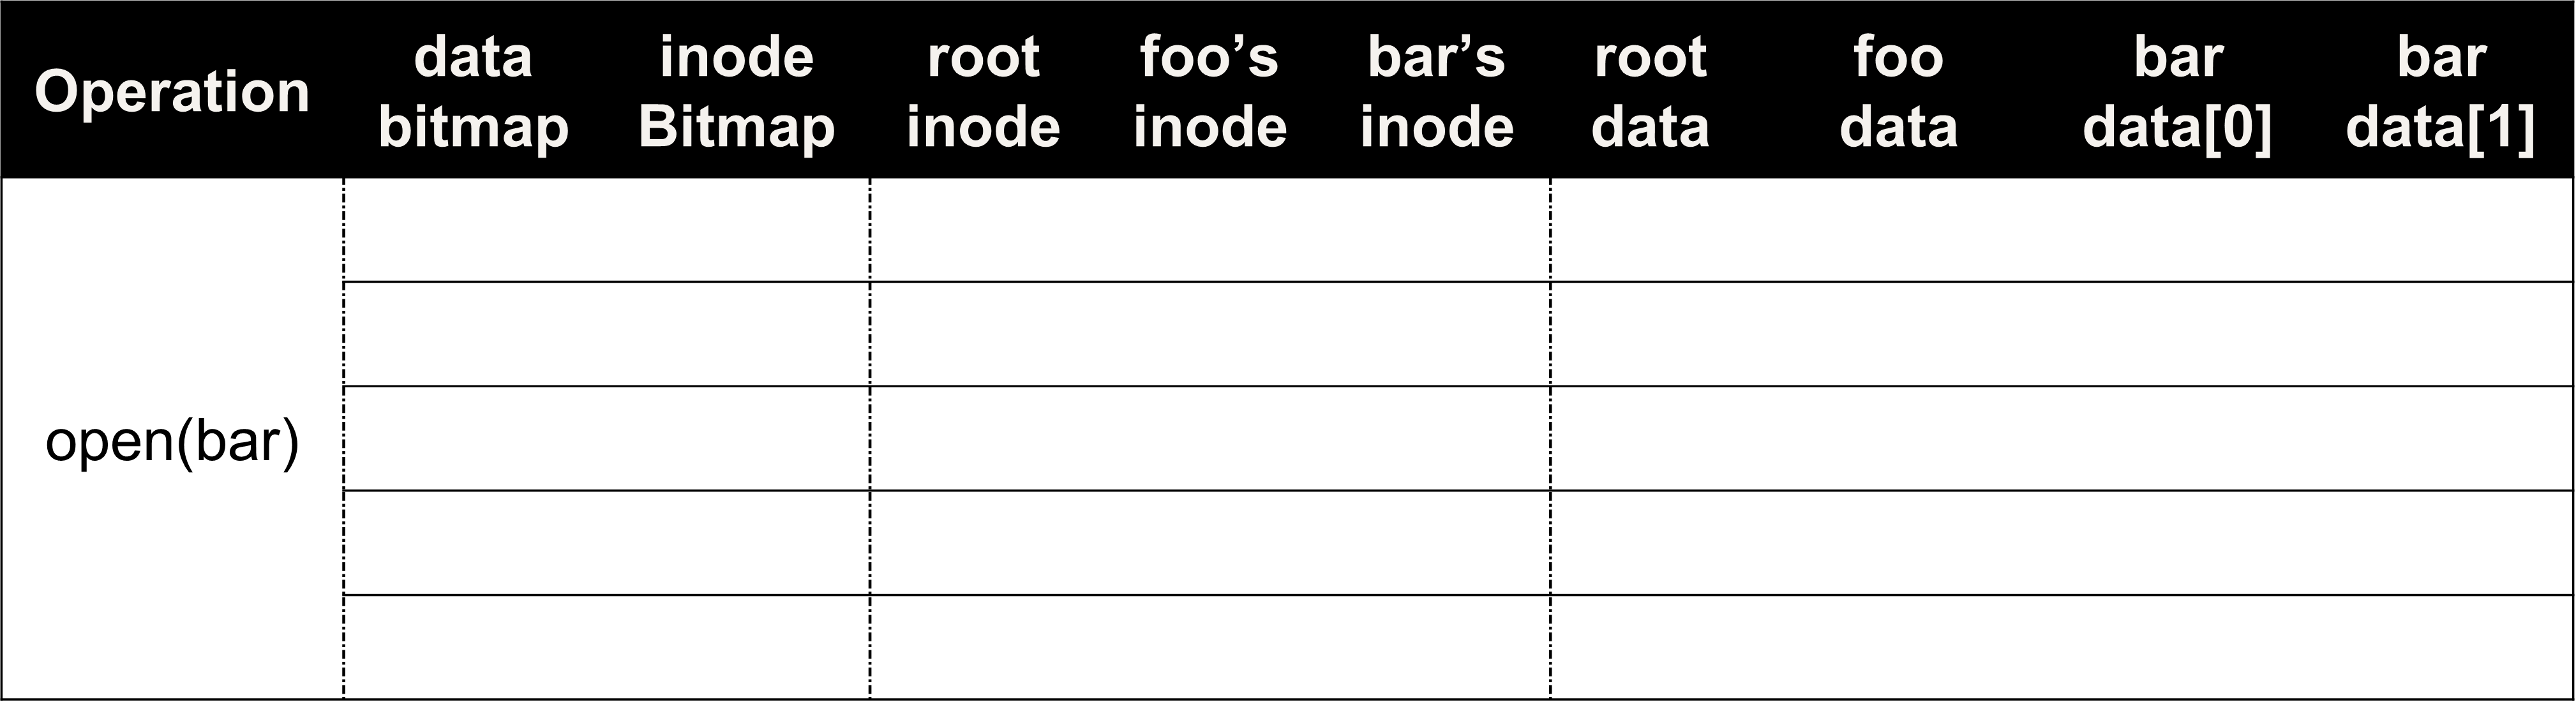
\includegraphics[width=120mm]{read-file-1.png}

\end{slide}

\begin{slide}

    \slidetitle{To read a file}

    Example: We want to read an 8 KB file /foo/bar
    \bigskip

    Now we have the file open.
    \bigskip

    Each block is 4 KB, we must perform read twice.
    \bigskip

    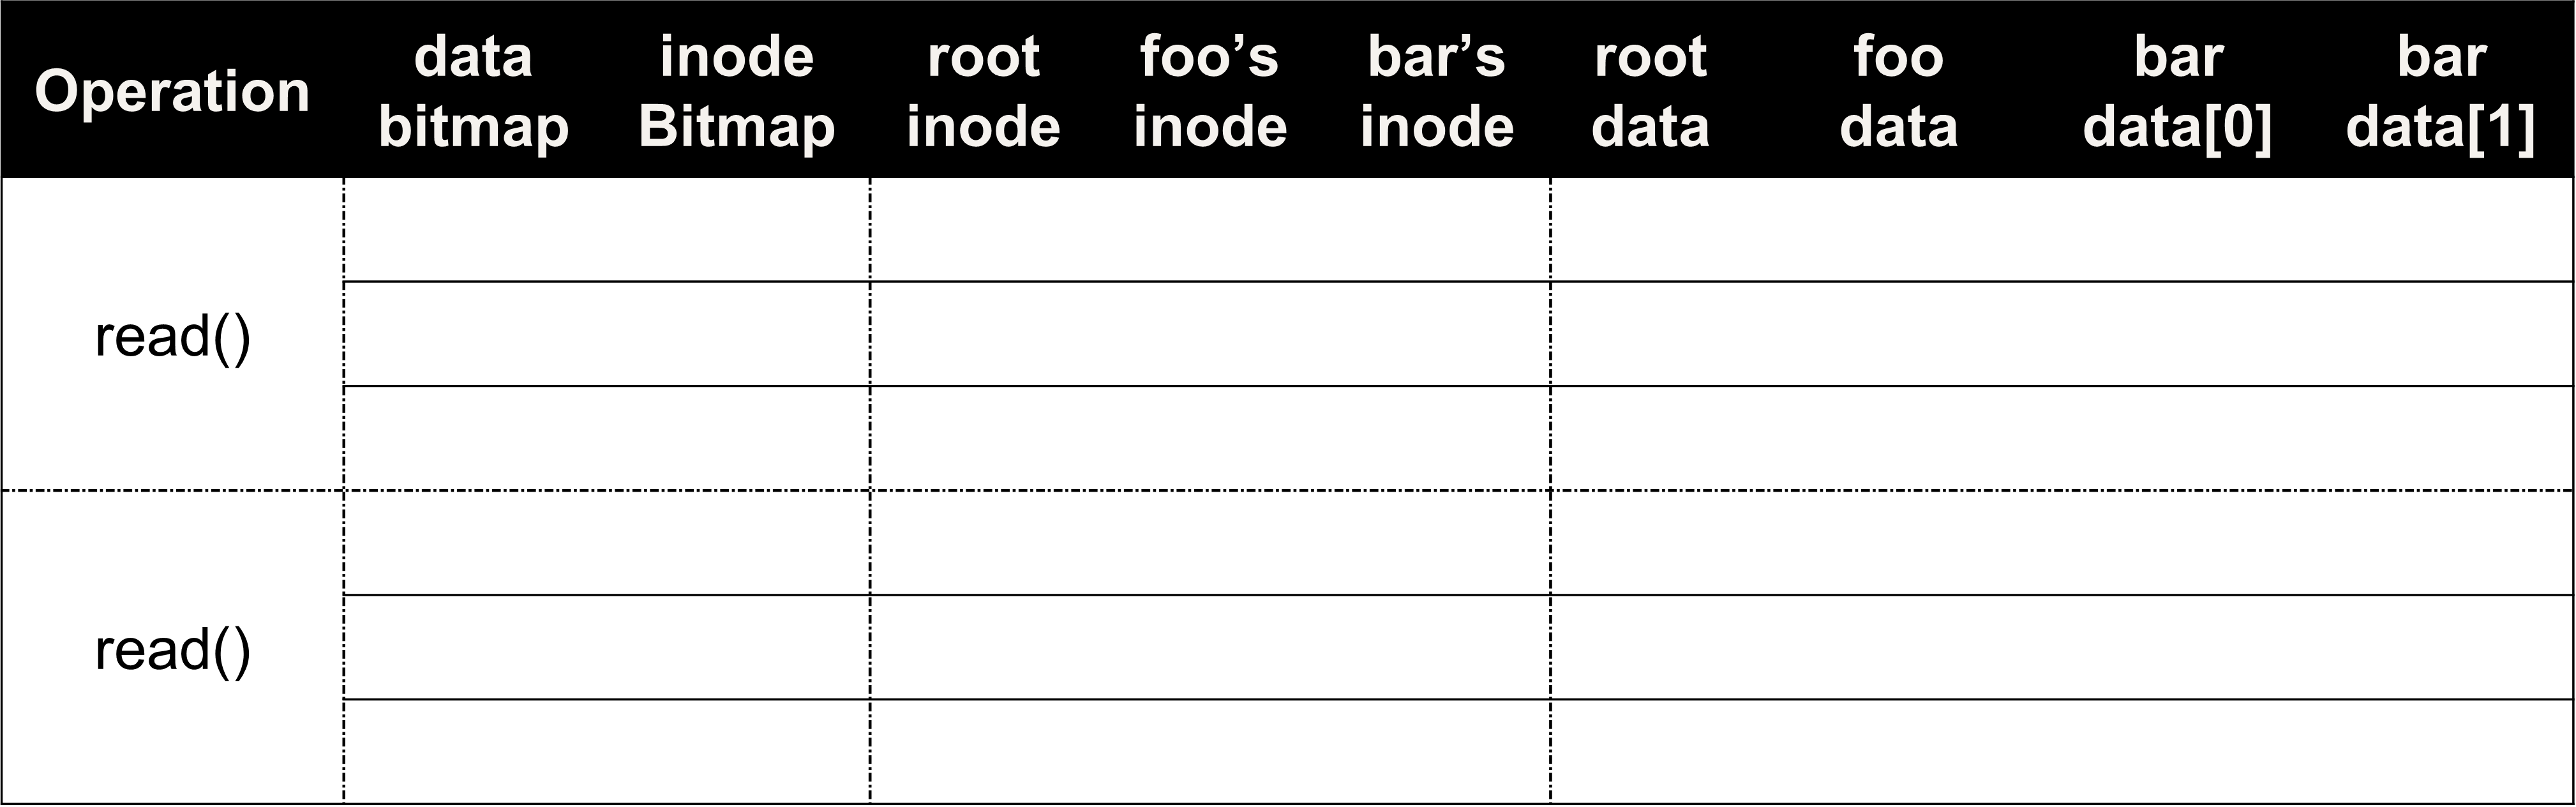
\includegraphics[width=120mm]{read-file-2.png}

\end{slide}

\begin{slide}

    \slidetitle{To write a file}

    \textbf{The high level idea}
    \begin{itemize}
        \item Similar to read – need to traverse the path to the file
        \item Unlike read – may need to allocate a file/block
        \item Block allocation updates multiple structures
    \end{itemize}
    \bigskip

    Example: We want to create and write to an 8 KB file /foo/bar

\end{slide}

\begin{slide}

    \slidetitle{To write a file}

    Example: We want to create and write to an 8 KB file /foo/bar
    \bigskip

    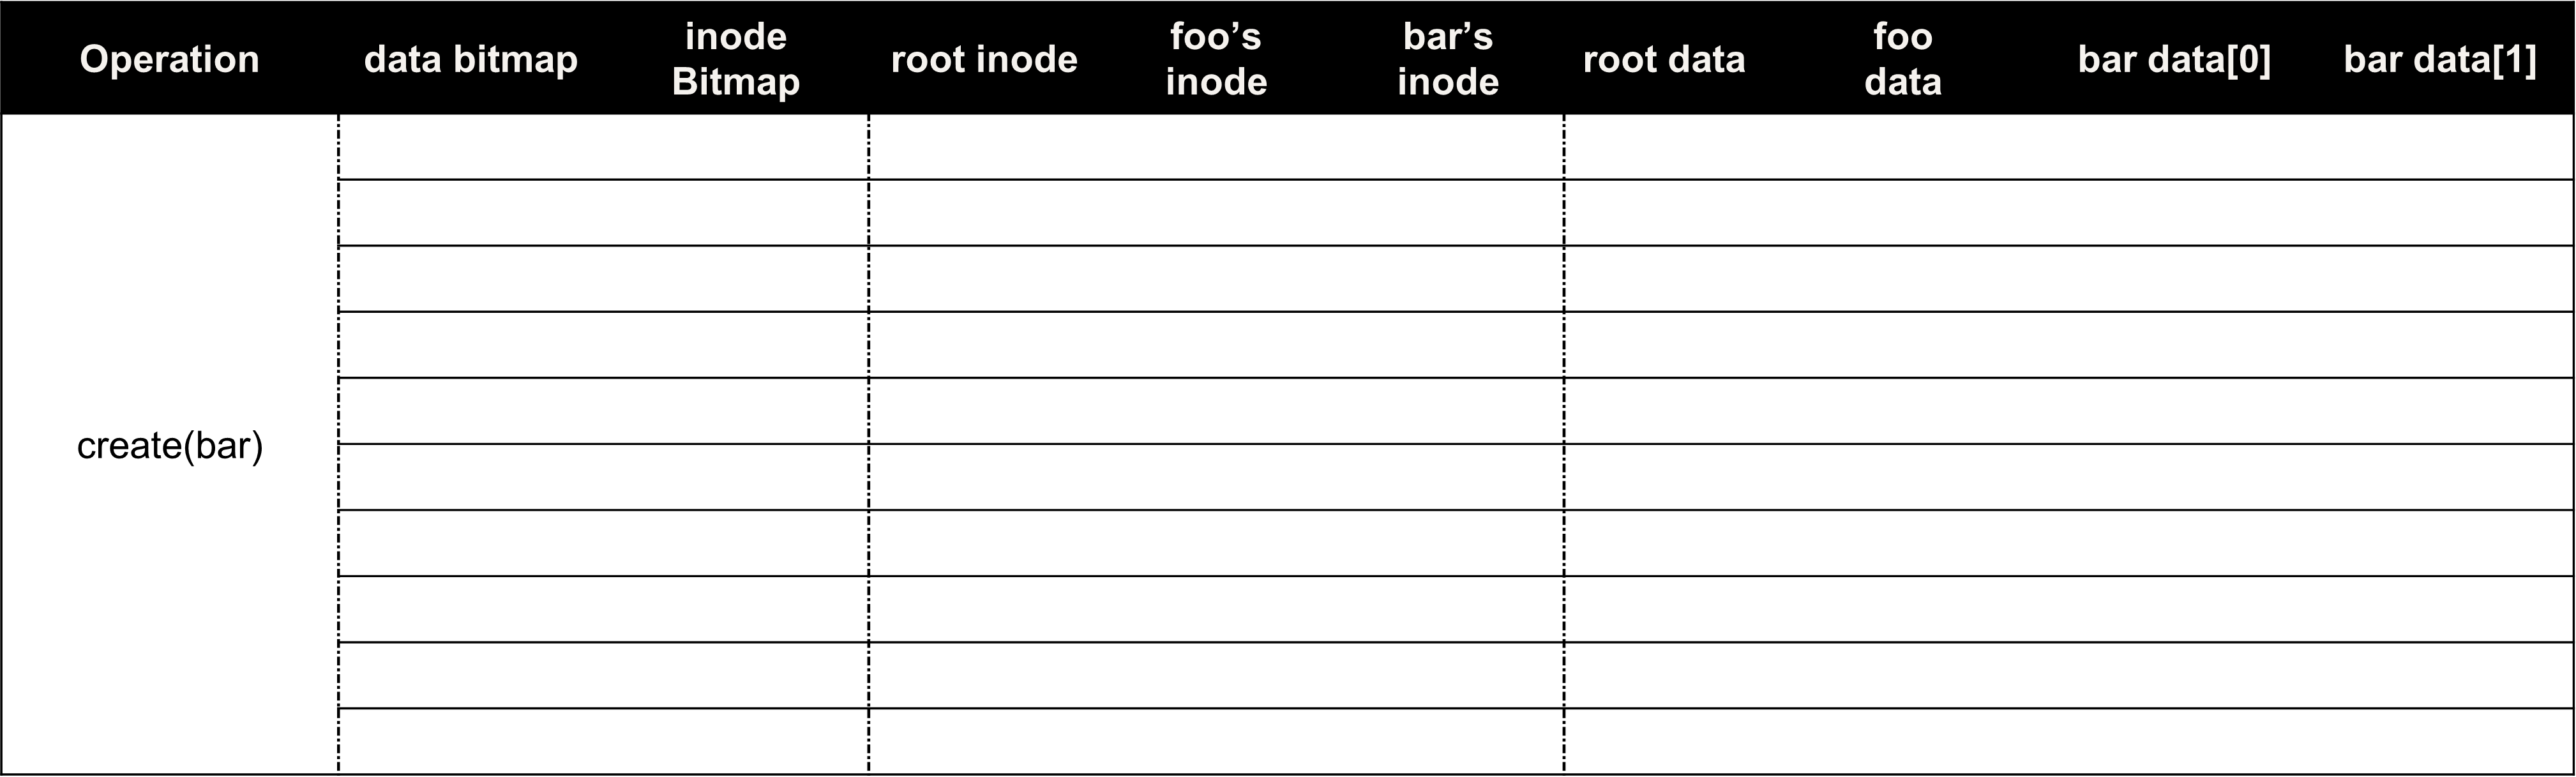
\includegraphics[width=130mm]{write-file-1.png}

\end{slide}

\begin{slide}

    \slidetitle{To write a file}

    Example: We want to create and write to an 8 KB file /foo/bar
    \bigskip

    File now exists but it is empty.
    \bigskip

    We need to perform 2 writes of 4 KB each.
    \bigskip

    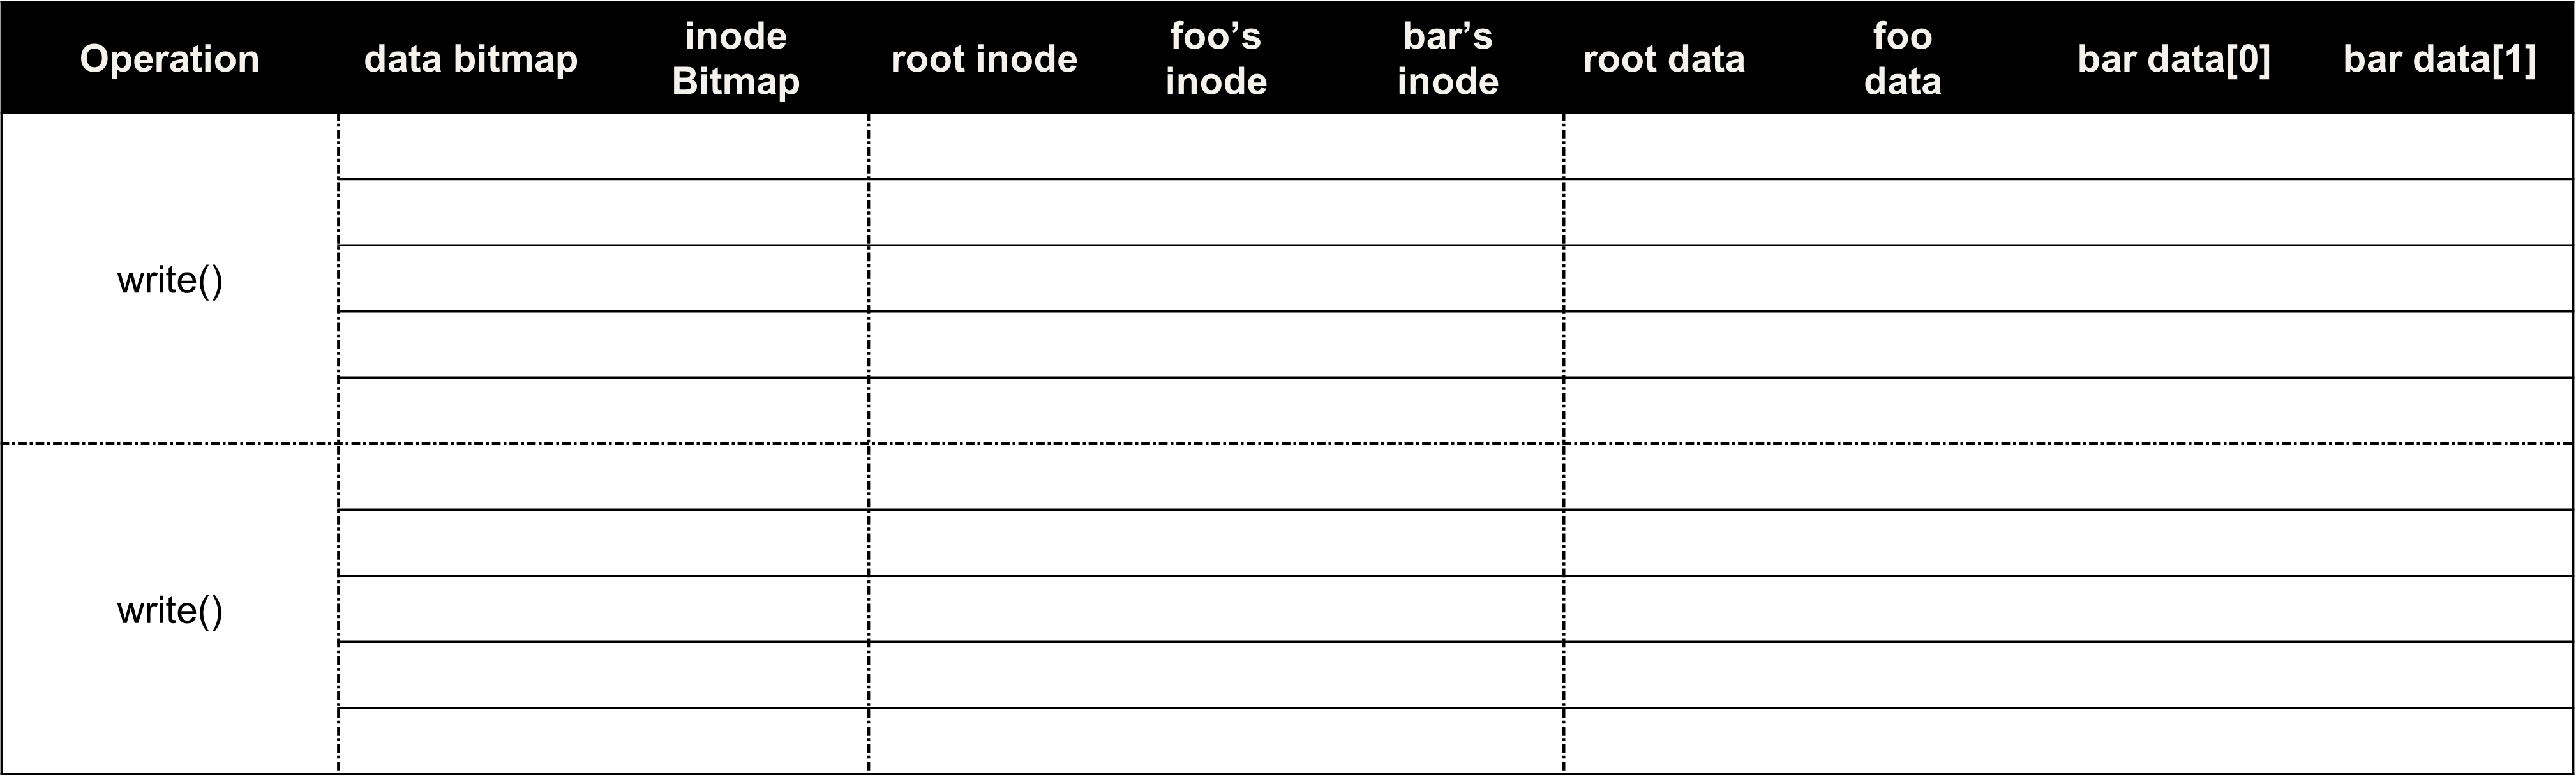
\includegraphics[width=130mm]{write-file-2.png}

\end{slide}

\begin{slide}

    \slidetitle{Sharing a file}

    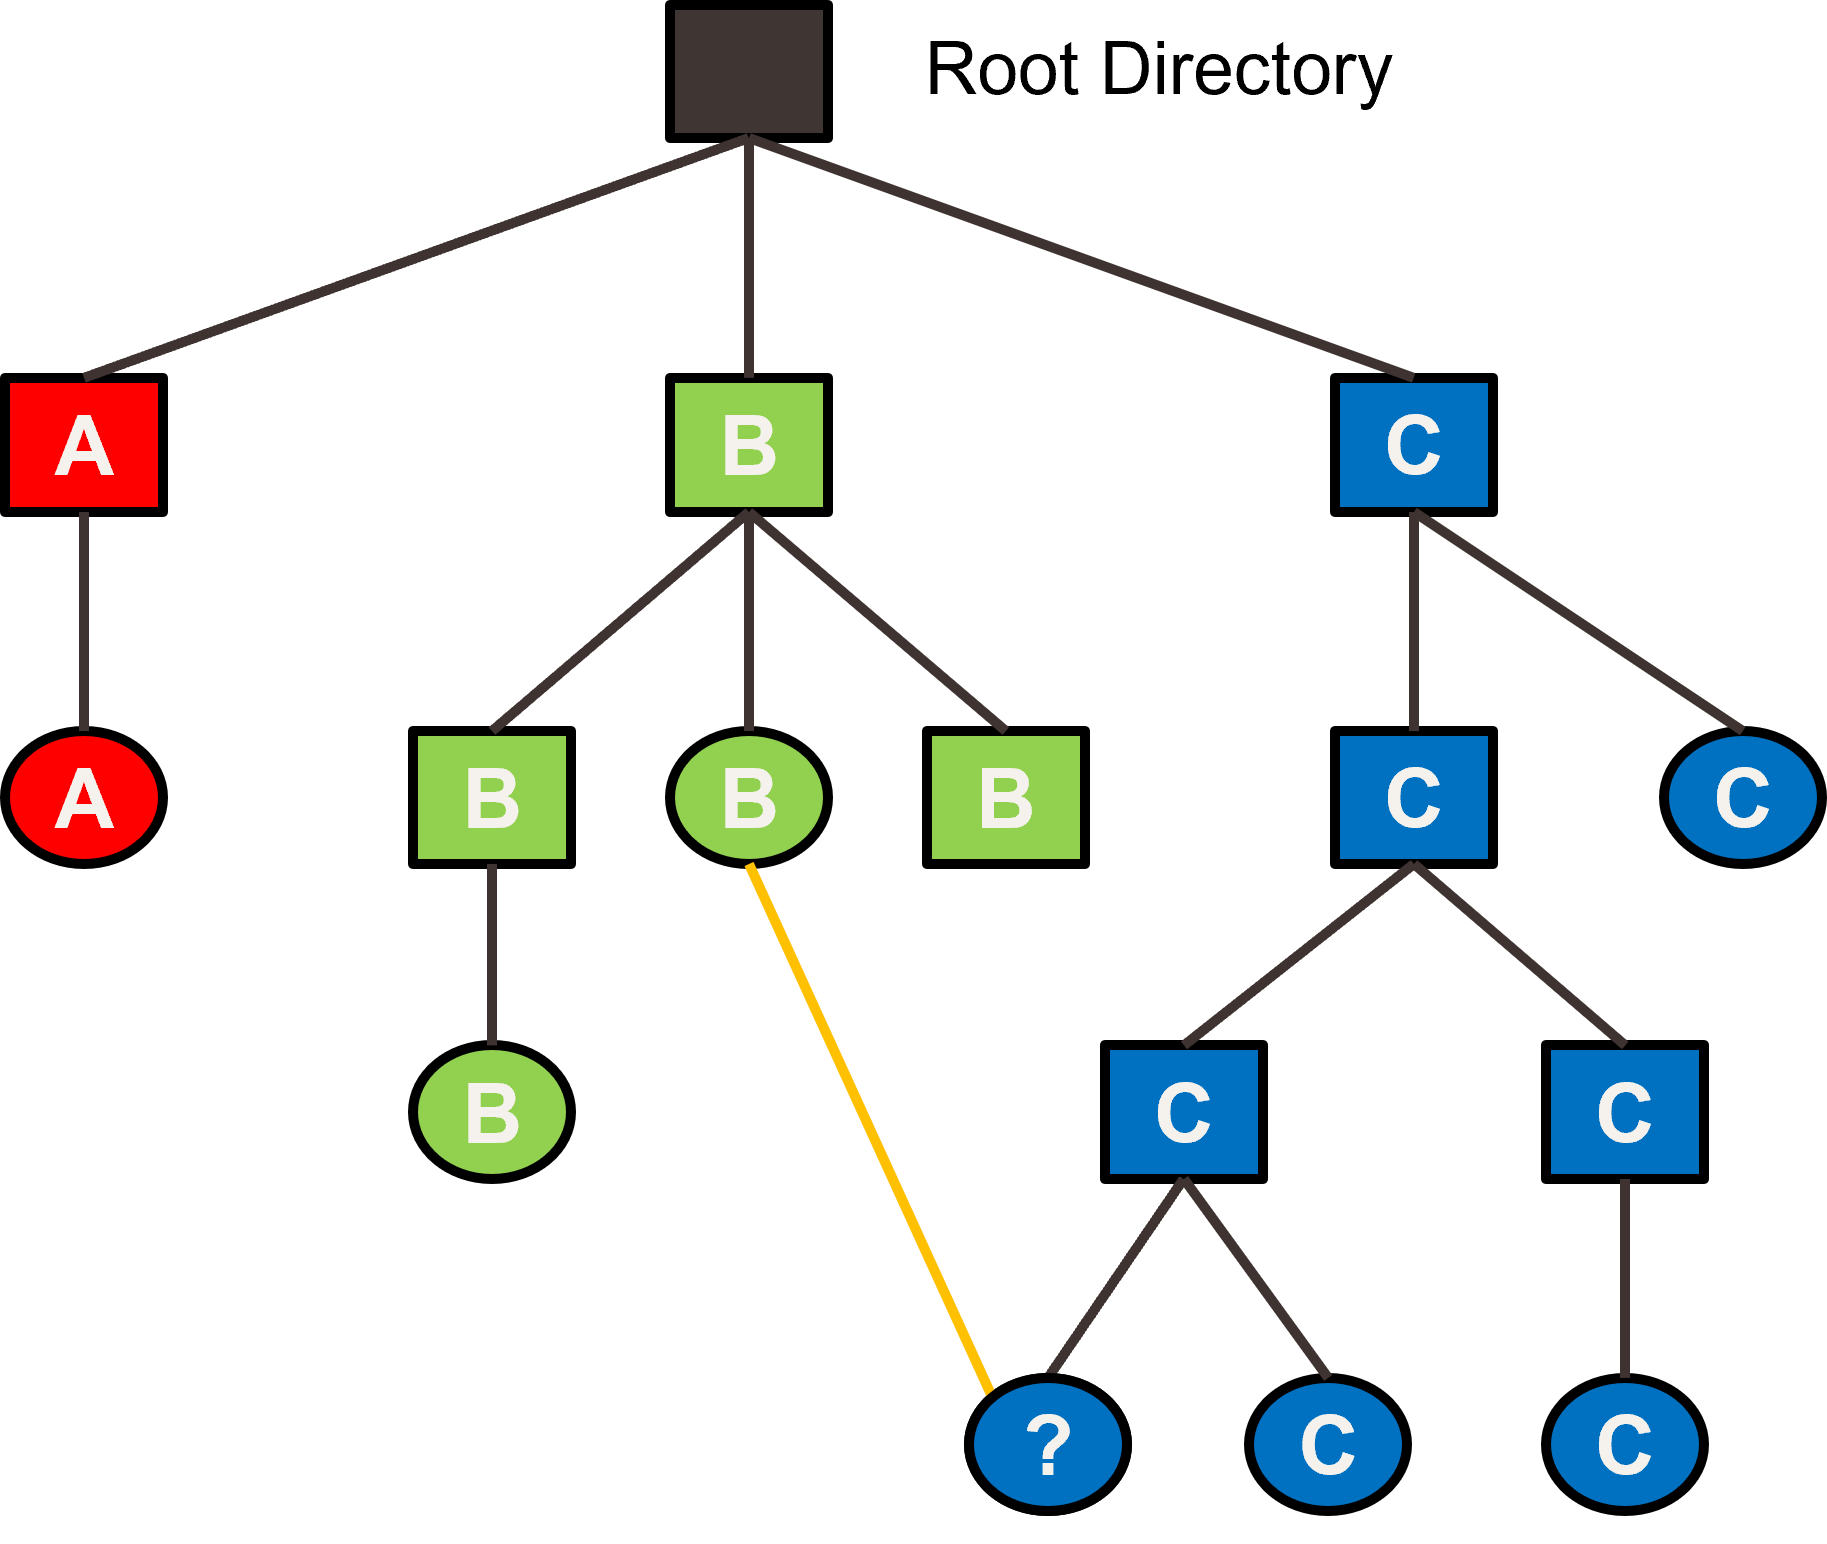
\includegraphics[width=50mm]{sharing-data-1.png}
    \bigskip

    What are the different ways User B and User C can share a file?

\end{slide}

\begin{slide}

    \slidetitle{Sharing a file}

    Hard Links are pointers to inodes.

    \medskip
    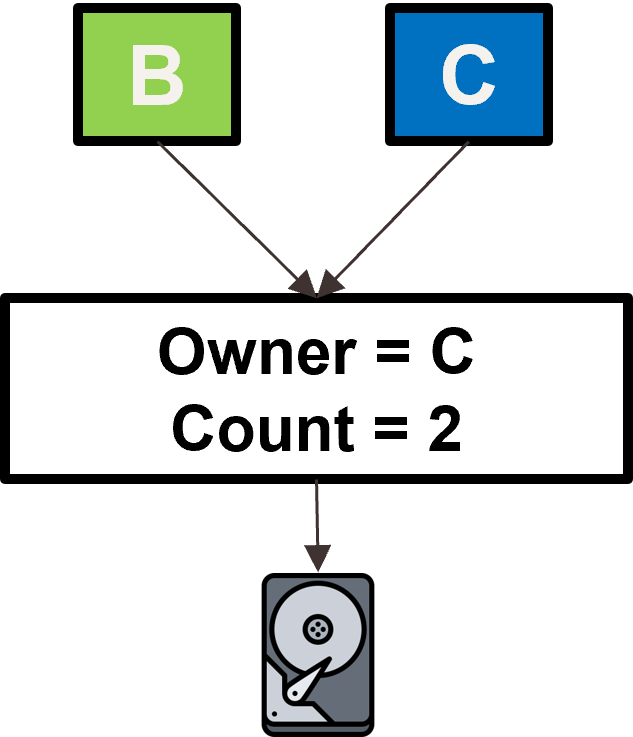
\includegraphics[width=22mm]{hard-link.png}
    \medskip

    Deleting a file only removes one hard link.
    
    The file can still be accessed

    \medskip
    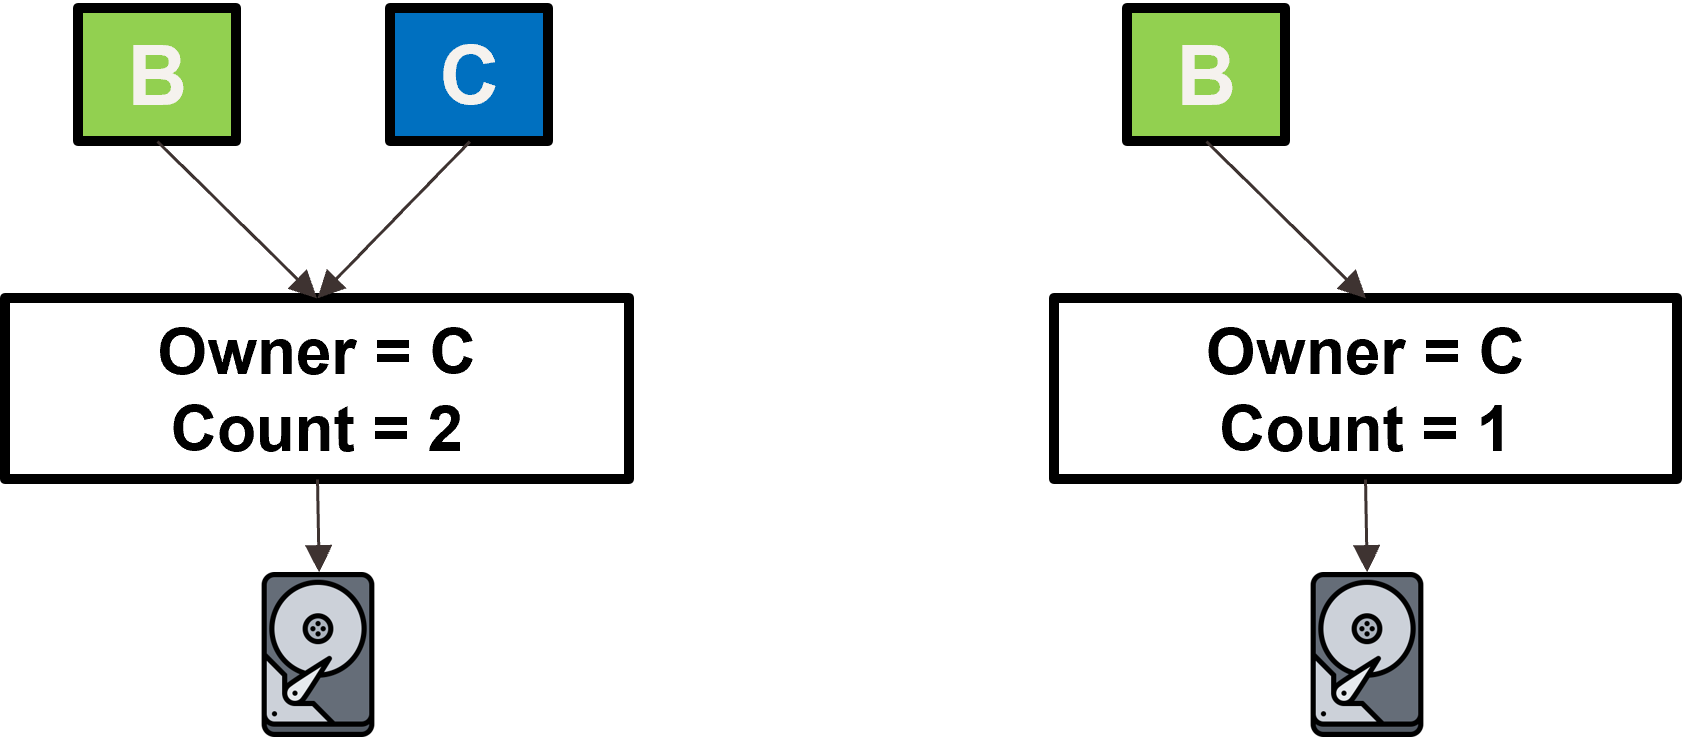
\includegraphics[width=55mm]{hard-link-removal.png}

\end{slide}

\begin{slide}

    \slidetitle{Sharing a file}

    Soft links are paths to another file.

    \medskip
    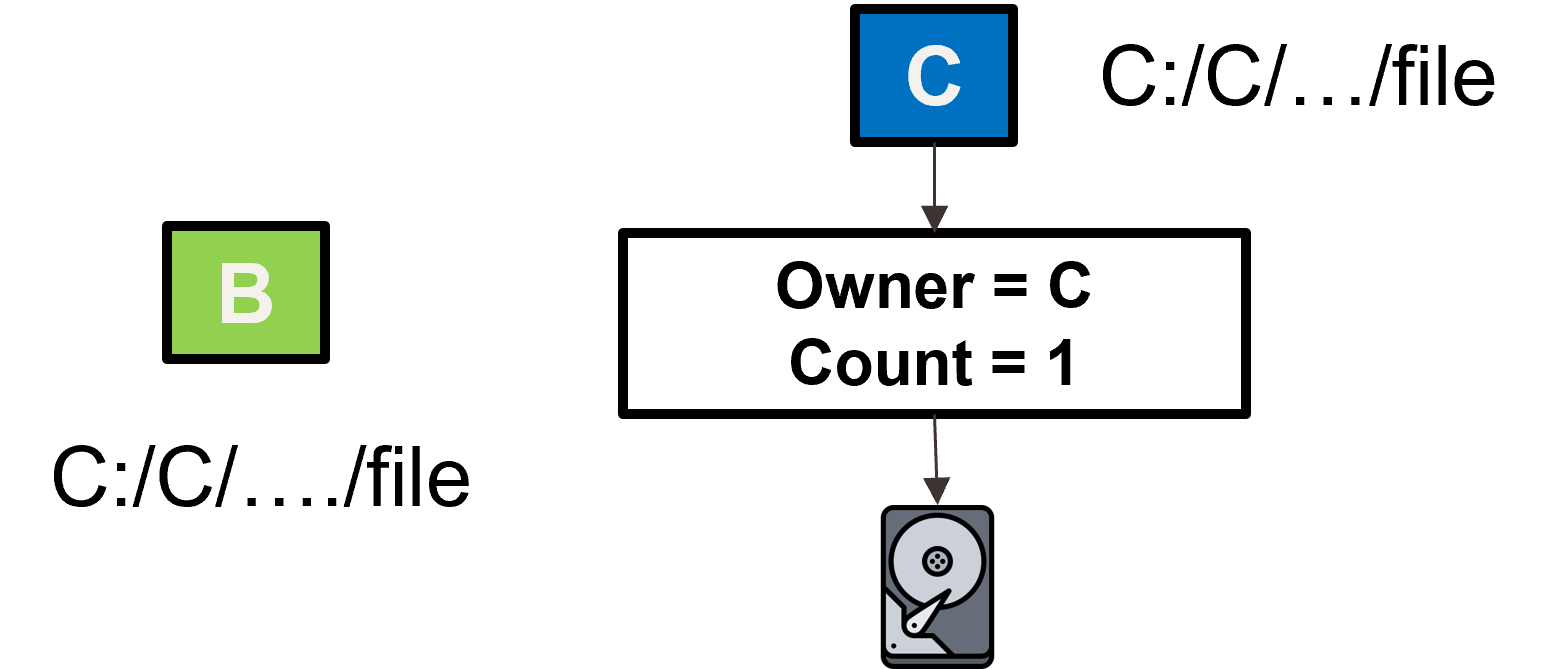
\includegraphics[width=75mm]{symbolic-link.png}
    \bigskip

    When resolving the file, the file system is redirected somewhere else, so: 
    \begin{itemize}
        \item Soft link targets do not need to exist 
        \item Soft link targets can be deleted without notice of the soft link 
        \item Unresolvable soft links lead to an exception
    \end{itemize}

\end{slide}

\begin{slide}

    \slidetitle{Cycles in Directory Graph}

    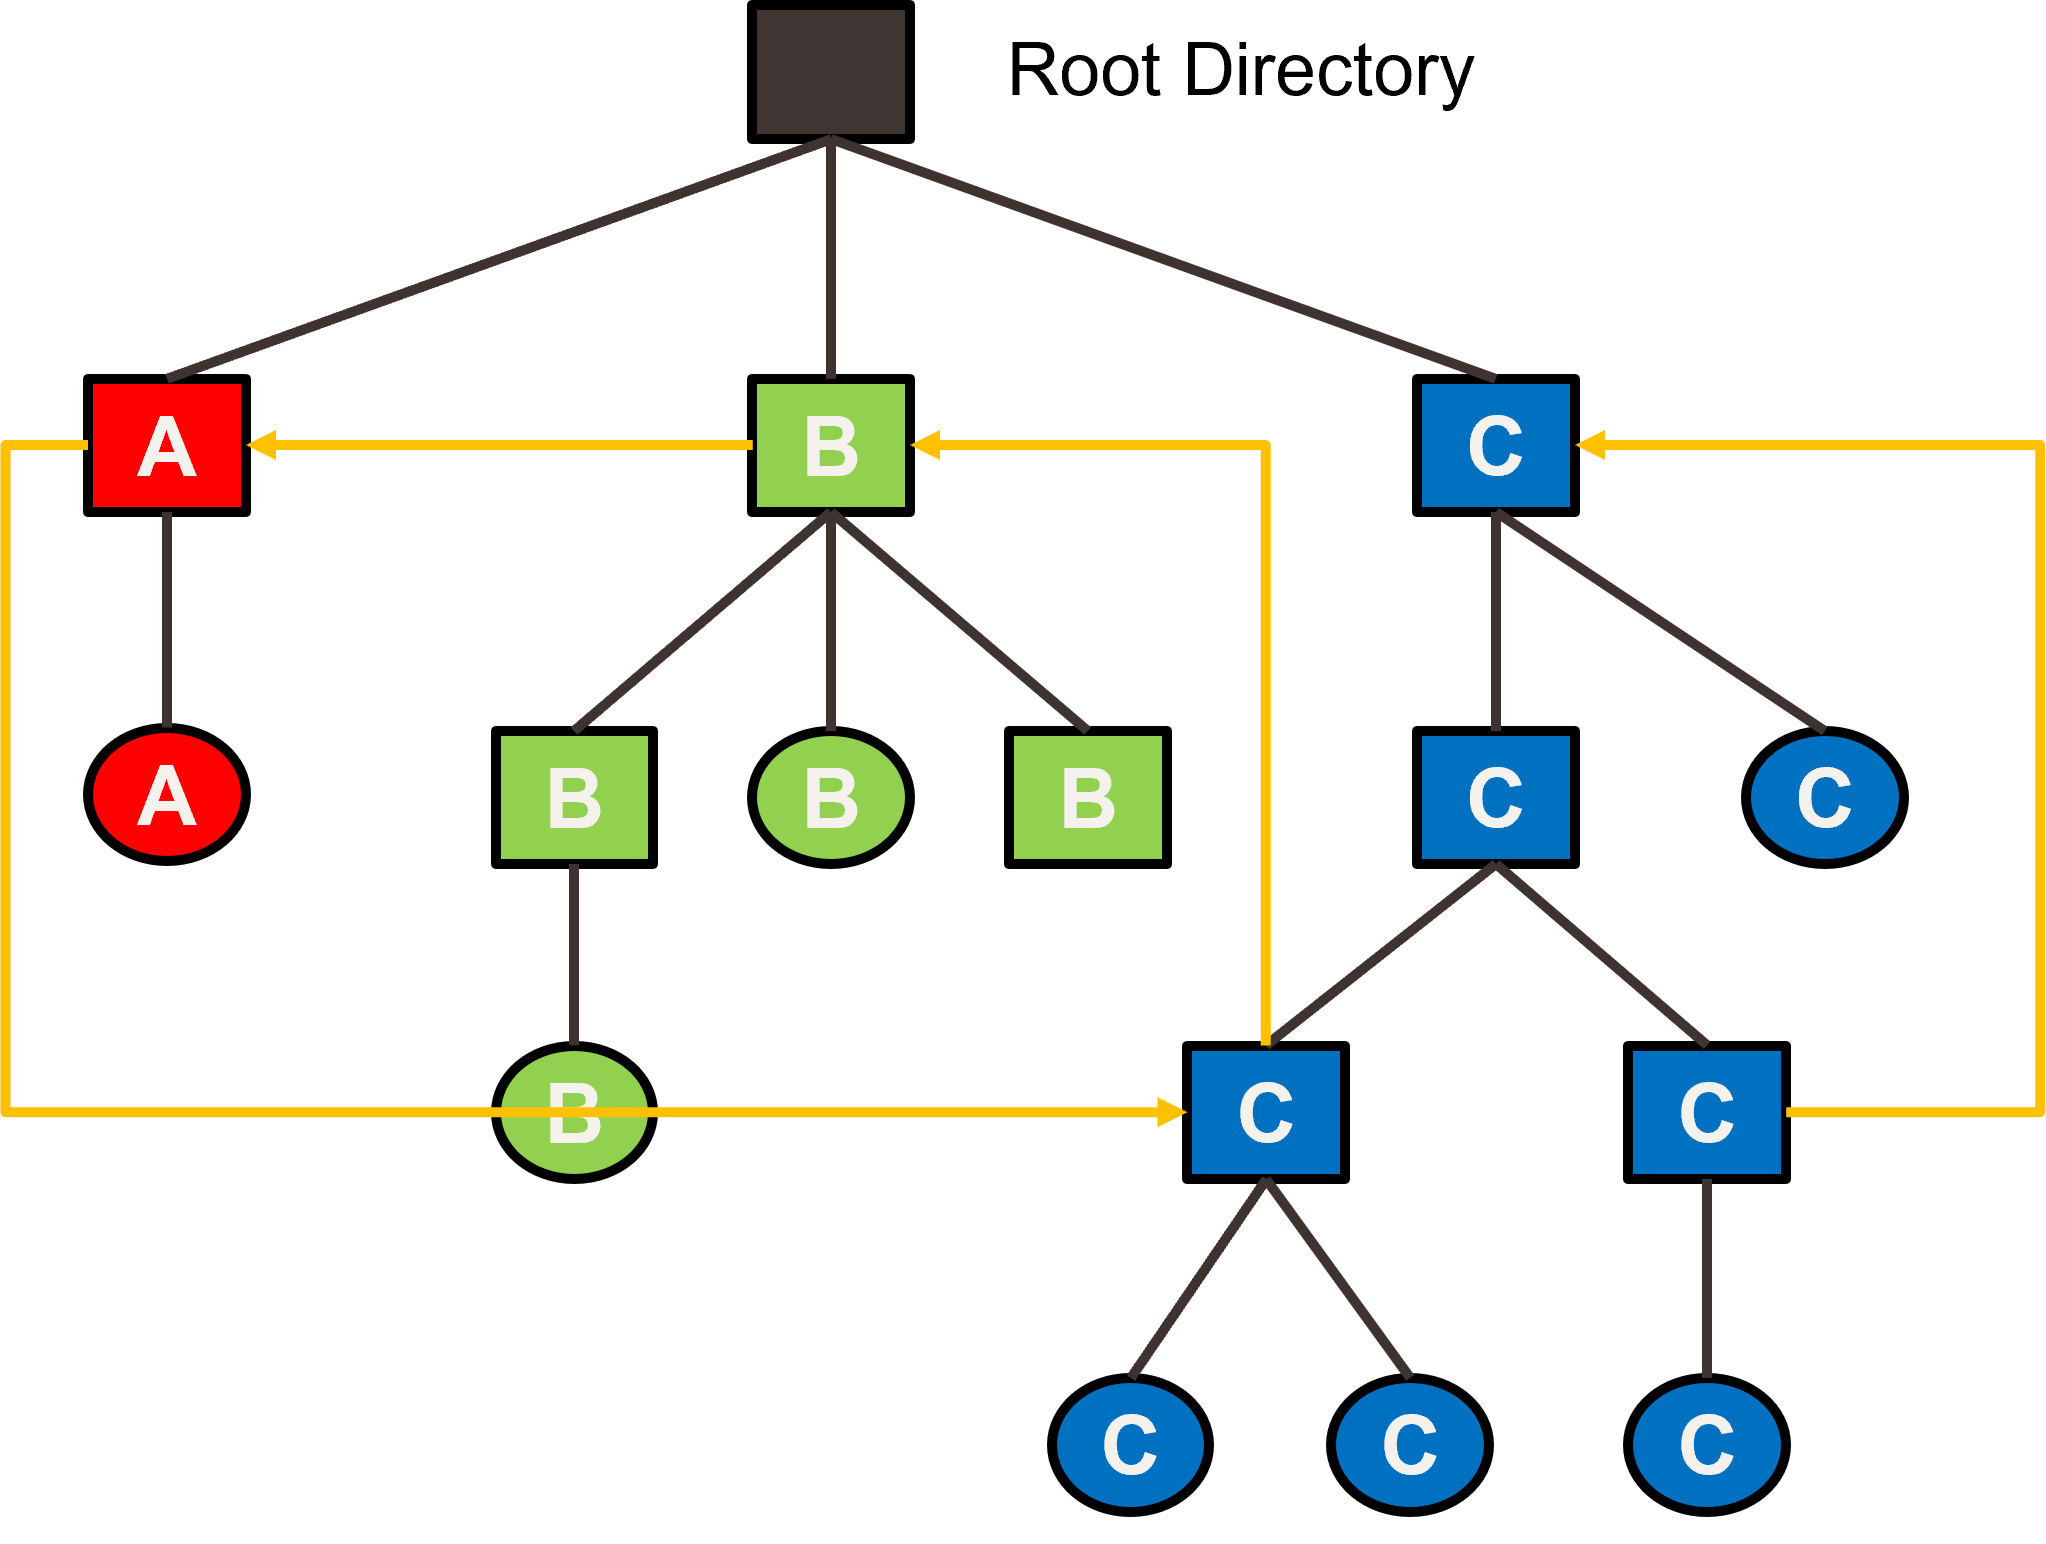
\includegraphics[width=60mm]{cycles-directory-graph.png}
    \bigskip

    Why are cyclic loops a problem?

    How do we solve this?

\end{slide}

\begin{slide}
    
    \slidetitle{Filesystem Example Problem}

    \begin{minted}{console}
touch todo.txt
ln todo.txt b.txt
ln -s todo.txt c.txt
mv todo.txt d.txt
rm b.txt
    \end{minted}
    \medskip

    How does the FS look like before and after the mv and rm commands?

\end{slide}

\begin{slide}
    
    \slidetitle{Filesystem Example Solution (1)}

    \begin{minted}{console}
touch todo.txt
ln todo.txt b.txt
ln -s todo.txt c.txt
mv todo.txt d.txt
rm b.txt
    \end{minted}
    \medskip

    Before mv:
    \medskip

    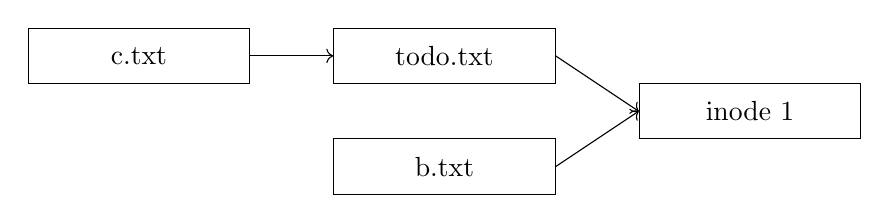
\begin{tikzpicture}[node distance=0mm and 0mm]
      \node[rectangle,draw,minimum width=80,minimum height=20] (inode1)   {inode 1};
      \node[rectangle,draw,minimum width=80,minimum height=20,xshift=-30,yshift=20] (fileA)  [left=of inode1] {todo.txt};
      \node[rectangle,draw,minimum width=80,minimum height=20,xshift=-30,yshift=-20] (fileB)  [left=of inode1] {b.txt};
      \node[rectangle,draw,minimum width=80,minimum height=20,xshift=-30] (fileC)  [left=of fileA] {c.txt};
  
      \draw[->] (fileA.east) -- (inode1.west);
      \draw[->] (fileB.east) -- (inode1.west);
      \draw[->] (fileC.east) -- (fileA.west);
    \end{tikzpicture}

\end{slide}

\begin{slide}
    
    \slidetitle{Filesystem Example Solution (2)}

    \begin{minted}{console}
touch todo.txt
ln todo.txt b.txt
ln -s todo.txt c.txt
mv todo.txt d.txt
rm b.txt
    \end{minted}
    \medskip

    After mv:
    \medskip

    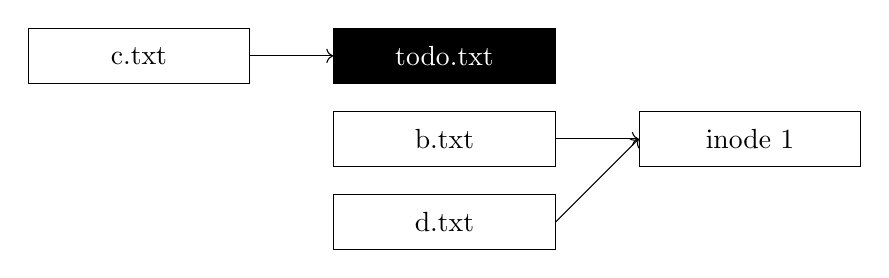
\begin{tikzpicture}[node distance=0mm and 0mm]

      \node[rectangle,draw,minimum width=80,minimum height=20] (inode1)   {inode 1};
      \node[rectangle,draw,minimum width=80,minimum height=20,xshift=-30,yshift=30,fill=black,text=white] (fileA)  [left=of inode1] {todo.txt};
      \node[rectangle,draw,minimum width=80,minimum height=20,xshift=-30] (fileB)  [left=of inode1] {b.txt};
      \node[rectangle,draw,minimum width=80,minimum height=20,xshift=-30,yshift=-30] (fileD)  [left=of inode1] {d.txt};
      \node[rectangle,draw,minimum width=80,minimum height=20,xshift=-30] (fileC)  [left=of fileA] {c.txt};
  
      \draw[->] (fileD.east) -- (inode1.west);
      \draw[->] (fileB.east) -- (inode1.west);
      \draw[->] (fileC.east) -- (fileA.west);
    \end{tikzpicture}

\end{slide}

\begin{slide}
    
    \slidetitle{Filesystem Example Solution (3)}

    \begin{minted}{console}
touch todo.txt
ln todo.txt b.txt
ln -s todo.txt c.txt
mv todo.txt d.txt
rm b.txt
    \end{minted}
    \medskip

    After rm:
    \medskip

    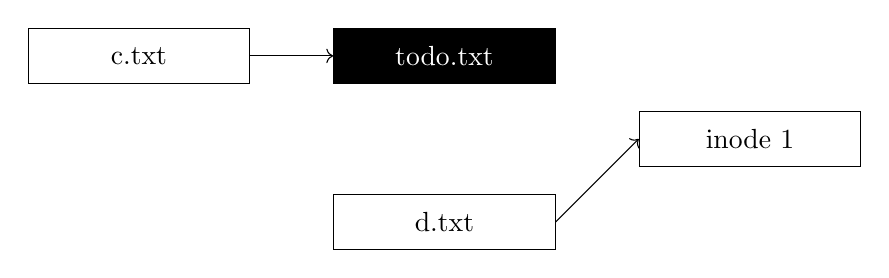
\begin{tikzpicture}[node distance=0mm and 0mm]
      \node[rectangle,draw,minimum width=80,minimum height=20] (inode1)   {inode 1};
      \node[rectangle,draw,minimum width=80,minimum height=20,xshift=-30,yshift=30,fill=black,text=white] (fileA)  [left=of inode1] {todo.txt};
      \node[rectangle,draw,minimum width=80,minimum height=20,xshift=-30,yshift=-30] (fileD)  [left=of inode1] {d.txt};
      \node[rectangle,draw,minimum width=80,minimum height=20,xshift=-30] (fileC)  [left=of fileA] {c.txt};
    
      \draw[->] (fileD.east) -- (inode1.west);
      \draw[->] (fileC.east) -- (fileA.west);
    \end{tikzpicture}

\end{slide}

\begin{slide}
    
    \slidetitle{What Data is Stored in an inode?}
    \small
    \begin{itemize}
        \item[a] Filename
        \item[b] Containing Directory name
        \item[c] File Size 
        \item[d] File type
        \item[e] \# of soft links to file
        \item[f] location of soft links 
        \item[g] \# of hard links to file  
        \item[h] location of hard links
        \item[i] access rights
        \item[j] timestamps
        \item[k] file contents
        \item[l] ordered list of data blocks     
    \end{itemize}
    
\end{slide}

\begin{slide}
    
    \slidetitle{What Data is Stored in an inode? Solution}
    \small
    \begin{itemize}
        \item[a] Filename \textit{No. Names are stored in directories}
        \item[b] Containing Directory name \textit{No. File can be in multiple dirs}
        \item[c] File Size \textit{Yes}
        \item[d] File type \textit{Yes}
        \item[e] \# of soft links to file \textit{No (they are unknown)}
        \item[f] location of soft links \textit{No (they are unknown)}
        \item[g] \# of hard links to file \textit{Yes (to know when to erase the file, check \texttt{stat})}
        \item[h] location of hard links \textit{No (they are unknown to the inode)}
        \item[i] access rights \textit{Yes}
        \item[j] timestamps \textit{Yes}
        \item[k] file contents \textit{Sometimes}
        \item[l] ordered list of data blocks \textit{Yes, by definition} 
    \end{itemize}

\end{slide}
  
\begin{slide}

    \slidetitle{Symbolic and Hard Links - More Practise}
    
	What is the output?
	\bigskip
	
    \begin{minted}[fontsize=\scriptsize, escapeinside=]{console}
1    $ echo "hello world" > my_file
2    $ cat my_file
3    $ ln -s my_file my_symbolic_link
4    $ ln my_file my_hard_link
5    $ cat my_symbolic_link
6    $ cat my_hard_link
7    $ rm my_file
8    $ cat my_symbolic_link
9    $ cat my_hard_link
10   $ cat my_file
11   $ echo "hello world again!" > my_file
12   $ cat my_symbolic_link
13   $ cat my_hard_link
    \end{minted}
    
\end{slide}
\end{document}
